

% Präambel
\documentclass[%
fontsize=12pt,					% Schriftgröße
paper=a4,						% Papierformat
twoside=false, 					% einseitiges (false) oder zweiseitiges (true) Dokument
listof=totoc, 					% Tabellen- und Abbildungsverzeichnis ins Inhaltsverzeichnis
bibliography=totoc,				% Literaturverzeichnis ins Inhaltsverzeichnis aufnehmen
titlepage, 						% Titlepage-Umgebung statt \maketitle
headsepline, 					% horizontale Linie unter Kolumnentitel
%abstracton,					% Überschrift beim Abstract einschalten, Abstract muss dazu in {abstract}-Umgebung stehen
DIV=12,							% Satzspiegeleinstellung, 12 ist Standar bei KOMA
BCOR=6mm,						% Bindekorrektur, die den Seitenspiegel um 3mm nach rechts verschiebt,
cleardoublepage=empty,			% Stil einer leeren eingefügten Seite bei Kapitelwechsel
parskip,							% Absatzabstand bei Absatzwechsel einfügen
ngerman
]{scrbook}			
\usepackage[setspace=false]{scrhack}
\usepackage[utf8]{inputenc} 	% ermöglicht die direkte Eingabe von Umlauten
\usepackage[T1]{fontenc} 		% Ausgabe aller zeichen in einer T1-Codierung (wichtig für die Ausgabe von Umlauten!)
\usepackage{babel} 	% deutsche Trennungsregeln und Übersetzung der festcodierten Überschriften
\renewcaptionname{ngerman}{\contentsname}{Inhaltsverzeichnis}
\renewcaptionname{ngerman}{\bibname}{Literaturverzeichnis}
\setlength{\parindent}{0ex} 	% bei neuem Abschnitt nicht einrücken
%------
% Folgende Einstellungen entsprechen den Vorgaben der Leitlinien
\usepackage[onehalfspacing]{setspace}
% Ende Leitlinien
%------
%------
% Folgende Einstellungen sind bei größeren Arbeiten mit viel Text zu empfehlen.
% Hierbei oben DIV=16 einstellen und Zeile \usepackage[onehalfspacing]{setspace} auskommentieren.
%\linespread{1.2}\selectfont     % Zeilenabstand erhöhen - größere Werte als 1.2 nicht verwenden!!
% Ende Einstellung große Arbeiten mit viel Text.
%------

\newcommand{\lowrule}{%
	\leavevmode \kern.06em\vbox{\hrule width.5em}}

\usepackage{siunitx}			% Vereinfachte Eingabe von Einheiten in Formeln
\sisetup{
	number-unit-product = \;,
	inter-unit-product = \:,
	exponent-product = \cdot,
	output-decimal-marker = {,}
}

\usepackage{graphicx}  			% Einbinden von Grafiken erlauben
\usepackage[format=hang,		% Formatierungen von Unter- / Überschriften
font=normal,
labelfont=bf,
justification=RaggedRight,
singlelinecheck=true,
aboveskip=1mm
]{caption}

\usepackage[backend=biber, %% Hilfsprogramm "biber" beim Compilieren nutzen (statt "biblatex" oder "bibtex")
style=alphabetic, %% Zitierstil (siehe Dokumentation)
natbib=true, %% Bereitstellen von natbib-kompatiblen Zitierkommandos
hyperref=true, %% hyperref-Paket verwenden, um Links zu erstellen
]{biblatex}
\setcounter{biburllcpenalty}{7000}
\setcounter{biburlucpenalty}{8000}
\addbibresource{literature/literatur1.bib} %% Einbinden der bib-Datei. Endung .bib unbedingt ergänzen
\addbibresource{literature/Manuelle.bib} %% Einbinden mehrerer bib-Dateien mit zusätzlichem \addbibresource - Befehl
\addbibresource{literature/T3Studienarbeit.bib}
\usepackage{csquotes}

% Folgende Zeilen sind auszukommentieren, falls runde Klammern und ein vgl. bei Zitaten erscheinen sollen.
%\makeatletter
%\renewcommand{\@cite}[2]{(vgl. {#1\if@tempswa , #2\fi})} 
%\renewcommand{\@biblabel}[1]{(#1)}
%\makeatother


\usepackage{float}
\usepackage{caption}
\usepackage{pdfpages}
\usepackage{tikz}
\usepackage{enumitem}			% Erlaubt Änderung der Nummerierung in der Umgebung enumerate
\usepackage{wrapfig}
\usepackage{amsmath}			% Ergänzungen für Formeln
\usepackage{textcomp} 			% zum Einsatz von Eurozeichen u. a. Symbolen
\usepackage{eurosym}			% bessere Darstellung Euro-Symbol mit \euro
\usepackage{amsfonts}
\usepackage{listings}
\usepackage{xcolor}
\usepackage[					% Einstellunge Paket hyperref
hyperfootnotes=false,			% im pfd-Output Fußnoten nicht verlinken
hidelinks						% Entfernen von farbigen Umrandungen der Links
]{hyperref}

\usepackage{makeidx}			% Paket zur Erstellung eines Index
\usepackage[toc]{glossaries}			% Paket zur Erstellung eines Glossars
\newglossaryentry{gls:glossar}
{
	name=Glossar,
	description={Als Glossar wird eine Liste von ausgewählten Begriffen bezeichnet, denen eine jeweilige Erläuterung zugeordnet ist. Ein Glossar wird, sofern gewünscht, im Anhang des Dokuments hinzugefügt.}
}
\usepackage[intoc]{nomencl} 			% zur Erstellung des Abkürzungsberzeichnisses

\usepackage[					% Einstellungen für Fußnoten
bottom,							% Ausrichtung unten
multiple,						% Trennung durch Seperator bei mehreren Fußnoten
hang,
marginal
]{footmisc}
\usepackage[utf8]{inputenc}
\usepackage{array}
\usepackage{colortbl}
\documentclass[a4paper,12pt]{article}
\usepackage{geometry}
\geometry{a4paper, margin=1in}
\usepackage{tikz}
\usepackage{amsmath}
\usepackage{calc}				% Paket zum Berechnen von Längen z.B. 0.8\linewidth

\usepackage{xcolor} 			% einfache Verwendung von Farben in nahezu allen Farbmodellen

\usepackage{multirow}
\usepackage{listings}			% Darstellung von Quellcode mit den Umgebungen {lstlisting}, \lstinline und \lstinputlisting
\lstset{literate=				% Damit können Umlaute innerhalb Listings geschrieben werden
	{Ö}{{\"O}}1
	{Ä}{{\"A}}1
	{Ü}{{\"U}}1
	{ß}{{\ss}}1
	{ü}{{\"u}}1
	{ä}{{\"a}}1
	{ö}{{\"o}}1
}
\definecolor{mygreen}{rgb}{0,0.6,0}
\definecolor{mygray}{rgb}{0.5,0.5,0.5}
\definecolor{mymauve}{rgb}{0.58,0,0.82}
\lstset{ %
	backgroundcolor=\color{white},   % choose the background color; you must add \usepackage{color} or \usepackage{xcolor}; should come as last argument
	basicstyle=\footnotesize,        % the size of the fonts that are used for the code
	breakatwhitespace=false,         % sets if automatic breaks should only happen at whitespace
	breaklines=true,                 % sets automatic line breaking
	captionpos=t,                    % sets the caption-position to (b) bottom or (t) top
	commentstyle=\color{mygreen},    % comment style
	deletekeywords={...},            % if you want to delete keywords from the given language
	escapeinside={\%*}{*)},          % if you want to add LaTeX within your code
	escapeinside={(*@}{@*)},
	extendedchars=true,              % lets you use non-ASCII characters; for 8-bits encodings only, does not work with UTF-8
	frame=none,	                   	% "single" adds a frame around the code; "none"
	keepspaces=true,                 % keeps spaces in text, useful for keeping indentation of code (possibly needs columns=flexible)
	keywordstyle=\color{blue},       % keyword style
	language=[LaTeX]TeX,             % the language of the code
	morekeywords={*,nomenclature},   % if you want to add more keywords to the set
	numbers=left,                    % where to put the line-numbers; possible values are (none, left, right)
	numbersep=5pt,                   % how far the line-numbers are from the code
	numberstyle=\tiny\color{mygray}, % the style that is used for the line-numbers
	rulecolor=\color{black},         % if not set, the frame-color may be changed on line-breaks within not-black text (e.g. comments (green here))
	showspaces=false,                % show spaces everywhere adding particular underscores; it overrides 'showstringspaces'
	showstringspaces=false,          % underline spaces within strings only
	showtabs=false,                  % show tabs within strings adding particular underscores
	stepnumber=1,                    % the step between two line-numbers. If it's 1, each line will be numbered
	stringstyle=\color{mymauve},     % string literal style
	tabsize=2,	                   % sets default tabsize to 2 spaces
	title=\lstname                   % show the filename of files included with \lstinputlisting; also try caption instead of title
}

\usepackage{float}


% -----------------------------------------------------------------------------------------------------------------
% Zum Aktualisieren des Abkürzungsverzeichnisses (Nomenklatur) bitte auf der Kommandozeile folgenden Befehl aufrufen :
% makeindex <Dateiname>.nlo -s nomencl.ist -o <Dateiname>.nls
% Oder besser: Kann in TexStudio unter Tools-Benutzer als Shortlink angelegt werden
% Konfiguration unter: Optionen-Erzeugen-Benutzerbefehle: makeindex -s nomencl.ist -t %.nlg -o %.nls %.nlo
% -----------------------------------------------------------------------------------------------------------------

% Hier die persönlichen Daten eingeben:

\newcommand{\titel}{Realisierung eines Vier-Gewinnt Roboter}
\newcommand{\untertitel} {Mithilfe von Lego Spike und Mirco Python }
\newcommand{\arbeit}{Studienarbeit T3\lowrule 3100}
\newcommand{\studiengang}{Elektrotechnik}
\newcommand{\studienrichtung}{Automation}
\newcommand{\studienschwerpunkt}{}
\newcommand{\autor}{Patrik Peters / Simon Gschell}
\newcommand{\bearbeitungszeitraum}{10.10.2024 - 13.06.2025}
\newcommand{\matrikelnr}{187 /0815}
\newcommand{\kurs}{TEA22}
%\newcommand{\firma}{Name des Dualen Partners (entfällt ggf. bei Studienarbeit)}
\newcommand{\abgabe}{\today}
\newcommand{\betreuerfirma}{Prof. Dr. ing Thorsten Kever}
%newcommand{\gutachterdhbw}{Gutachterin / Gutachter der DHBW (nur bei Bachelorarbeit)}

\newcommand{\jahr}{2019}			% für Angabe im Copyright-Vermerk der Titelseite

% Folgende Zeilen definieren Abkürzungen, um Befehle schneller eingeben zu können
\newcommand{\ua}{\mbox{u.\,a.\ }}
\newcommand{\zB}{\mbox{z.\,B.\ }}
\newcommand{\bs}{$\backslash$}
\newcommand*\diff{\mathop{}\!\mathrm{d}}	% Differentialzeichen
\newcommand*\Diff[1]{\mathop{}\!\mathrm{d^#1}} % Differentialzeichen höherer Ableitung
\newcommand*\jj{\mathop{}\!\mathrm{j}}	% Komplexe Zahl j

% Folgende Zeilen weden benötigt, um Tikz und PGF-Plot-Grafiken einzubinden
\usepackage{pgfplots}
\usepackage{pgfplotstable}
\pgfplotsset{compat=newest,width=0.6\linewidth}
\usepgfplotslibrary{smithchart}
\usepackage{tikz}						% Tikz sollte nach Listings Pakete geladen werden.
\usetikzlibrary{arrows}

\hyphenation{Schrift-ar-ten}

%\BeforeClosingMainAux{% siehe KOMA-Script-Anleitung
%\addcontentsline{toc}{chapter}{\indexname}\stepcounter{page}
%}

%\makeindex						% Indexverzeichnis erstellen
\makenomenclature				% Abkürzungsverzeichnis erstellen
\makeglossaries

% -------------------------------------------------------------------------------------------
%                     Beginn des Dokumenteninhalts
% -------------------------------------------------------------------------------------------
\begin{document}
\let\texteuro\euro						% Eingabe \texteuro, € oder \euro erzeugt gleiches Ergebnis
\setcounter{secnumdepth}{3}				% Nummerierungstiefe fürs Inhaltsverzeichnis
\setcounter{tocdepth}{3}
\sffamily								% für die Titelei serifenlose Schrift verwenden

% ------------------------------ Titelei -----------------------------------------------------

\thispagestyle{plain}
\hypersetup{pageanchor=false}
\begin{titlepage}
\enlargethispage{4.0cm}
\sffamily 								% Serifenlose Grundschrift für die Titelseite einstellen

\parbox{0.5\linewidth}{
\begin{flushleft}
% Hier ggf. ein Logo der Firma
\end{flushleft}
}
\parbox{0.5\linewidth}{
\begin{flushright}
	
\includegraphics[width=0.4\linewidth]{images/DHBW_d_R_FN_46mm_4c}\\[5ex]
\end{flushright}
}
				

\begin{center}

{\fontsize{20.74pt}{24pt}\selectfont
\textbf{\titel}\\[1.5ex]}
{\fontsize{14pt}{17pt}\selectfont
\textbf{\untertitel}\\[5ex]}
{\fontsize{17pt}{20pt}\selectfont
\textbf{\arbeit}\\[2ex]}
{\fontsize{14pt}{17pt}\selectfont
Studiengang \studiengang\\[2ex]}
{\fontsize{12pt}{14pt}\selectfont
Studienrichtung \studienrichtung\\[1ex]
Duale Hochschule Baden-Württemberg Ravensburg, Campus Friedrichshafen\\[5ex]
von\\[1ex]
\autor\\[15ex]}


\end{center}

\begin{flushleft}
{\fontsize{12pt}{14pt}\selectfont
\begin{tabular}{ll}
Abgabedatum:					& \quad \abgabe \\
Bearbeitungszeitraum:		   	& \quad \bearbeitungszeitraum   \\ 
Matrikelnummer: 			& \quad \matrikelnr \\ 
Kurs: 							& \quad \kurs \\
%Dualer Partner:	 			& \quad \firma \\ % entfällt bei Studienarbeit
Betreuerin / Betreuer:  & \quad \betreuerfirma \\ % Betreuerin / Betreuer der Arbeit
%Gutachterin / Gutachter: & \quad \gutachterdhbw \\ [2ex] % Gutachterin / Gutachter der DHBW (nur bei der Bachelorarbeit erforderlich)
\end{tabular}
}
\end{flushleft}
%%%%% Nachfolgende Zeilen einkommentieren, wenn Copyrightvermerk gewünscht ist
%\begin{flushleft}
%{\fontsize{11pt}{13pt}\selectfont
%Copyrightvermerk:\\
%Dieses Werk einschließlich seiner Teile ist \textbf{urheberrechtlich geschützt}. Jede Verwertung außerhalb der engen Grenzen des Urheberrechtgesetzes ist ohne Zustimmung des Autors unzulässig und strafbar. Das gilt insbesondere für Vervielfältigungen, Übersetzungen, Mikroverfilmungen sowie die Einspeicherung und Verarbeitung in elektronischen Systemen.
%}
%\end{flushleft}
%\begin{flushright}
%{\fontsize{11pt}{13pt}\selectfont \copyright{} \jahr }
%\end{flushright}
\end{titlepage}

\ifthenelse{\boolean{@twoside}}{%
	\cleardoublepage
}{%
	\clearpage
}%

\hypersetup{pageanchor=true}
 				% erzeugt die Titelseite
\pagenumbering{roman}					% kleine, römische Seitenzahlen für Titelei
%% Ggf. folgende Zeile auskommentieren, falls der Sperrvermerk gewünscht ist.
%\chapter*{Sperrvermerk} %*-Variante sorgt dafür, das der Sperrvermerk nicht im Inhaltsverzeichnis auftaucht
%gemäß Ziffer 1.1.14 der Anlage 1 zu §§ 3, 4 und 5  der Studien- und Prüfungsordnung für die Bachelorstudiengänge im Studienbereich Technik der Dualen Hochschule Baden-Württemberg vom 29.09.2017 in der Fassung vom 24.07.2023:
%
%Der Inhalt dieser Arbeit darf weder als Ganzes noch in Auszügen Personen außerhalb des Prüfungsprozesses und des Evaluationsverfahrens zugänglich gemacht werden, sofern keine anders lautende Genehmigung vom Dualen Partner vorliegt.
%
%Musterstadt, den \today \\[4ex]
%
%\rule[-0.2cm]{5cm}{0.5pt} \\
%
%\textsc{\autor} \\[10ex]

\chapter*{Erklärung} %*-Variante sorgt dafür, dass die Erklärung nicht im Inhaltsverzeichnis auftaucht

gemäß Ziffer 1.1.14 der Anlage 1 zu §§ 3, 4 und 5  der Studien- und Prüfungsordnung für die Bachelorstudiengänge im Studienbereich Technik der Dualen Hochschule Baden-Württemberg vom 29.09.2017 in der Fassung vom 24.07.2023.

Wir versichern hiermit, dass wir unsere \arbeit\ mit dem Thema:

\begin{quote}
	\textit{\titel} % -\textit{ \untertitel }
\end{quote}

selbstständig verfasst und keine anderen als die angegebenen Quellen und Hilfsmittel benutzt haben. Wir versicheren zudem, dass die eingereichte elektronische Fassung mit der gedruckten Fassung übereinstimmt.\\[6ex]

Friedrichshafen, den \today \\[1ex]

\rule[-0.2cm]{10cm}{0.5pt} \\

\autor \\[10ex]

\rmfamily

\thispagestyle{empty}

 				% Einbinden der eidestattlichen Erklärung
\chapter*{Kurzfassung} %*-Variante sorgt dafür, das Abstract nicht im Inhaltsverzeichnis auftaucht

In der vorliegenden Studienarbeit wird die Entwicklung eines Roboters für das Spiel „Vier gewinnt“ unter Verwendung des LEGO Spike Prime Systems behandelt. Ziel des Projekts ist es, einen Roboter zu entwerfen, der in der Lage ist, autonom die Rolle eines menschlichen Gegners im Spiel „Vier gewinnt“ zu übernehmen. Der Roboter soll nicht nur die Spielzüge des menschlichen Mitspielers erkennen und darauf reagieren, sondern auch selbstständig Spielsteine in das Spielfeld einwerfen und sicherstellen, dass das Spielfeld für den nächsten Zug bereit ist. Dies erfordert eine präzise Steuerung des Roboters, insbesondere beim Platzieren der Spielsteine, sowie die Fähigkeit, das Spielfeld zu überwachen, um die Position der bereits gesetzten Steine zu erkennen.
Das Projekt umfasst verschiedene technische und organisatorische Aspekte. Dazu gehört die mechanische Konstruktion des Roboters, einschließlich des Mechanismus zum Einwerfen der Spielsteine und die Überwachung des Spielfelds, sowie die Entwicklung der Software, die die Spielzüge und das Verhalten des Roboters steuert. Ein weiterer wichtiger Punkt ist die Sensorik: Der Roboter muss in der Lage sein, die aktuelle Spielsituation durch Farbsensoren zu erfassen, um zu wissen, welche Felder im Spielfeld bereits besetzt sind und wo er seinen nächsten Spielstein platzieren kann.
Zum Abschluss des Projekts wird ein kleines Turnier organisiert, bei dem die von verschiedenen Teams entwickelten Roboterlösungen gegeneinander antreten. Dies bietet die Möglichkeit, den Roboter unter realen Bedingungen zu testen und seine Fähigkeiten im direkten Vergleich mit den Lösungen der anderen Kommilitonen zu messen. Um zusätzliche Motivation zu schaffen, wird die beste Lösung am Ende prämiert, was den Wettbewerbsgedanken fördert und den Anreiz erhöht eine effektive Lösungen zu entwickeln.

\clearpage

\chapter*{Abstract} %*-Variante sorgt dafür, das Abstract nicht im Inhaltsverzeichnis auftaucht
This student research project deals with the development of a robot for the game “Four Wins” using the LEGO Spike Prime system. The aim of the project is to design a robot that is capable of autonomously assuming the role of a human opponent in the game “Four Wins”. The robot should not only recognize the moves of the human opponent and react to them, but also independently place pieces on the playing field and ensure that the playing field is ready for the next move. This requires precise control of the robot, especially when placing the pieces, as well as the ability to monitor the playing field in order to recognize the position of the pieces already placed.
The project involves various technical and organizational aspects. These include the mechanical design of the robot, including the mechanism for inserting the tiles and monitoring the playing field, as well as the development of the software that controls the moves and behavior of the robot. Another important point is the sensor technology: the robot must be able to detect the current game situation using color sensors in order to know which squares in the playing field are already occupied and where it can place its next piece.
At the end of the project, a small tournament is organized in which the robot solutions developed by different teams compete against each other. This offers

Translated with DeepL.com (free version)
\clearpage   			% Einbinden des Abstracts

\tableofcontents						% Erzeugen des Inhalsverzeichnisses

\clearpage

% --------------------------------------------------------------------------------------------
%                    Inhalt der Bachelorarbeit
%---------------------------------------------------------------------------------------------
\pagenumbering{arabic}					% arabische Seitenzahlen für den Hauptteil

\rmfamily



\chapter{Einleitung}
\label{cha:Einleitung}

%Folgende Stichworte können zum Aufbau der Einleitung herangezogen werden.
%
%\begin{itemize}
%\item Hinführung, Begründung, Zweck und Ziel der Aufgabenstellung
%\item Erläuterung der Problemstellung
%\item Konkretisierung der zu lösenden Aufgabe
%\item Gegebenenfalls Formulierung einer Leitfrage oder Forschungsfrage
%\item Ausgangslage, geplante Vorgehensweise, Methoden zur Bearbeitung und Zielsituation
%\item Zum Ende der Einleitung wird eine Kurzübersicht über die Inhalte der Kapitel gegeben: \glqq Die Arbeit ist wie folgt gegliedert: ...\grqq
%\end{itemize}
%
%Die Einleitung wird üblicherweise auf ein bis zwei Seiten als fortlaufender Text geschrieben. Eine weitere Untergliederung in nummerierte Abschnitte ist nicht empfehlenswert, da dies erstens unüblich ist, zweitens die Lesbarkeit nicht begünstigt und drittens die Formulierung der Einleitung erschwert. Weitere Empfehlungen zum Aufbau der Einleitung und des gesamten Dokuments sind z.~B. aus \autocite{DHBW.2021} und \autocite{Lindenlauf.2022} zu entnehmen.
%
%\clearpage
%
%Hinweise: 
%
%\begin{itemize}
%\item Auch in der Einleitung unbedingt zu wichtigen Hintergründen und Fakten Zitate aufführen.\index{Zitat} Zitate bitte in der Form \autocite{Tipler.2019} oder mit Seitenbezug \autocite[66]{Ziegler.2017} oder auch mehrere Zitate  \autocite{Tipler.2019, Ziegler.2017} innerhalb einer eckigen Klammer angeben. Zur besseren Lesbarkeit bitte immer ein Leerzeichen vor dem Zitat einfügen.
%	
%\item Bereits in der Einleitung können Abkürzungen erläutert werden. Grundsätzlich gilt, dass bei der ersten Verwendung einer Abkürzung diese auch erläutert wird. Zum Beispiel können das Antiblockiersystem (ABS) oder die Fahrdynamikregelung (Electronic Stability Control, ESC) als Abkürzungen eingeführt werden. In der Datei \textit{pages/abkuerzungen.tex} sind alle verwendeten Abkürzungen einzufügen. Neben dem verpflichtenden Abkürzungsverzeichnis kann auch ein Glossar hinzugefügt werden. In dieser Vorlage können Glossareinträge in der Datei \textit{pages/glossar.tex} eingefügt werden. Ein \Gls{gls:glossar} ist jedoch nicht verpflichtend.
%\end{itemize}

Strategiespiel sind Spiele, welche nach einer Spieltheorie ablaufen.
$"$Vier-Gewinnt$"$, ist ein Gesellschafts- und Strategiespiel. Das Prinzip des Spiels ist recht einfach. Ein Teilnehmer beginnt, anschließend ist der andere Spieler am Zug.  Gewonne  hat der Teilnhemer, der zuesrt das Ziel erreicht bzw erfüllt hat.
\chapter{Grundlagen des Spiels Vier Gewinnt}
Im Kapitel Grundlagen wird auf die Regeln des Spiels, sowie auf den geschichtlichen Hintergrund als auch die mathematischen Eigenschaften des Spiels 4Gewinnt genauer eingegangen. 

\section{Spielregeln und Spielablauf}
%Die Regeln für dieses Strategiespiel sind kinderleicht, was auch ein Argument für die große Beliebtheit bei Jung und Alt ist. Das Spiel besteht aus einem senkrecht stehenden Spielbrett und jeweils aus 21 gelben und roten runde Steine. Diese Steine werden abwechselnd in das hohle Spielbrett mit 42 Aussparungen, sieben Spalten und sechs Reihen, eingeworfen. Der Spieler kann somit eine Spalte auswählen und den Stein fallen lassen. Der eingeworfene Stein besetzt den untersten freien Platz dieser Spalte. Das Spiel wird dann gewonnen, wenn einer der Spieler vier oder mehr Steine in einer waagerechten, senkrechten oder diagonalen Reihe platzieren kann. Der andere Spieler hat somit automatisch verloren. Kommt es zu keiner Bildung einer dieser Kombinationen, endet das Spiel bei Vergabe aller Steine in einem Remis.

Das originale Spiel 4Gewinnt besteht aus einer Rasterwand mit sechs Zeilen und sieben Spalten, also 42 Löchern. Außerdem besteht es aus 21 roten Spielchips und 21 gelben Spielchips. 4Gewinnt lässt sich nur zu zweit spielen. Ziel des Spieles ist es, vier Spielchips einer Farbe in eine Reihe (waagrecht, senkrecht oder diagonal) zu bringen. Der jüngste Spieler beginnt das Spiel. Der Spieler, der an der Reihe ist, wirft einen Spielstein seiner Farbe durch die Öffnung der Rasterwand, wo durch der gespielte Stein auf den untersten freien Platz in der Spalte fällt. Danach ist der andere Spieler an der Reihe. Die Spieler werfen so lange ihre Spielchips in das Raster, bis einer das Ziel erreicht hat oder alle 42 Felder belegt sind. Für den Fall, dass alle 42 Felder des Rasters belegt sind, endet das Spiel unentschieden. Um ein neues Spiel zu starten, muss ein Spieler die Steine aus dem Raster fallen lassen. Diese werden dann wieder unter den Spielern aufgeteilt und eine neue Runde 4Gewinnt kann beginnen\autocite{Hasbro.2020}.

\begin{figure}[H]
	\centering
	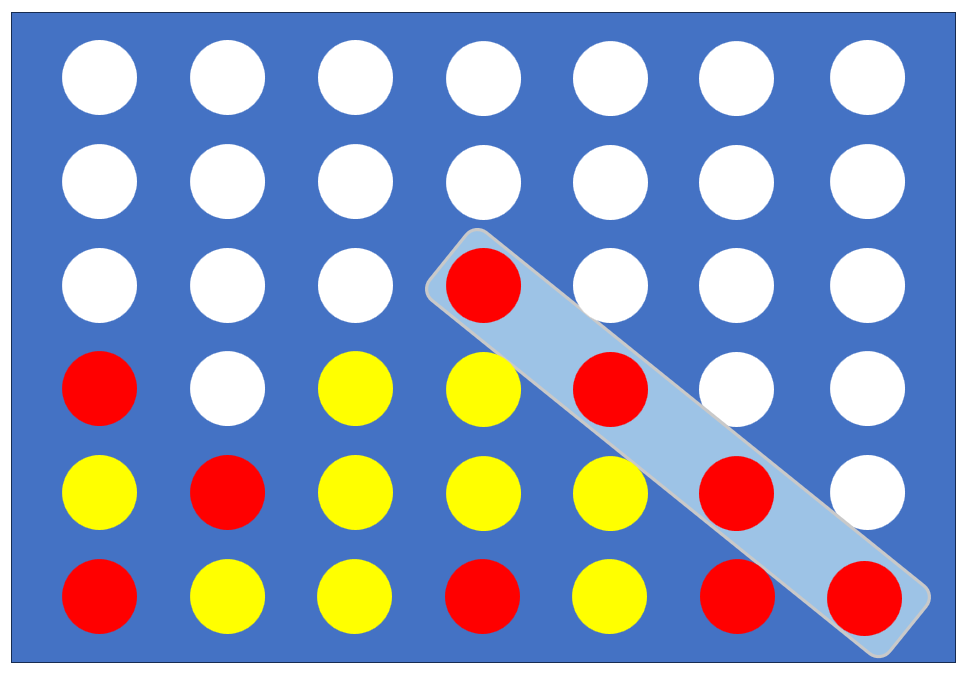
\includegraphics[width=0.8\linewidth]{images/Diagonal}
	\caption[Vier rote Steine diagonal]{Vier rote Steine diagonal im Raster}
	\label{fig:diagonal}
\end{figure}
\begin{figure}[H]
	\centering
	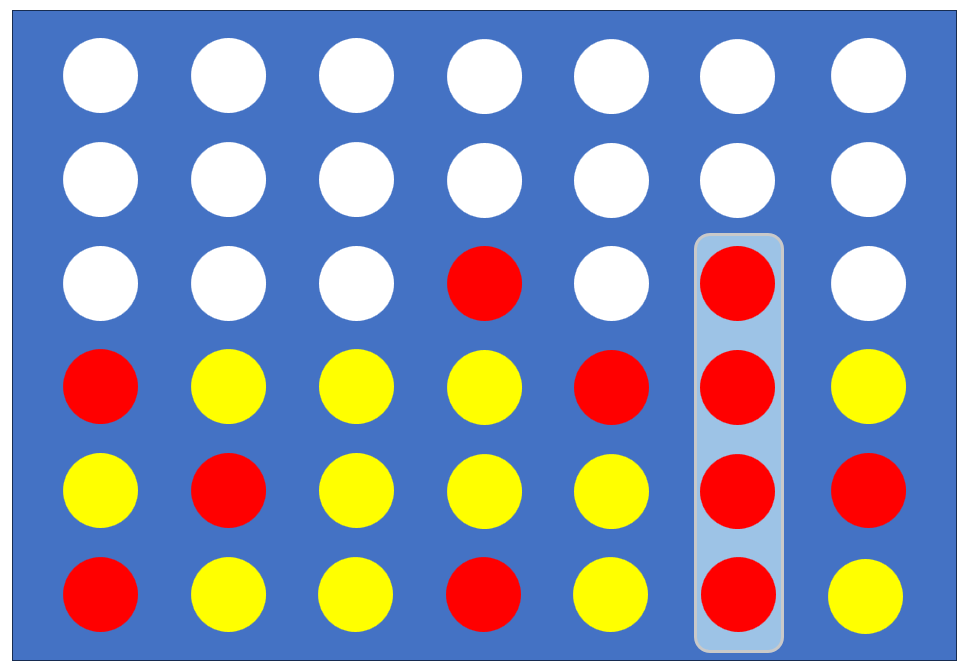
\includegraphics[width=0.8\linewidth]{images/Senkrecht}
	\caption[Vier rote Steine in Reihe senkrecht]{Vier rote Steine senkrecht im Raster}
	\label{fig:senkrecht}
\end{figure}
\begin{figure}[H]
	\centering
	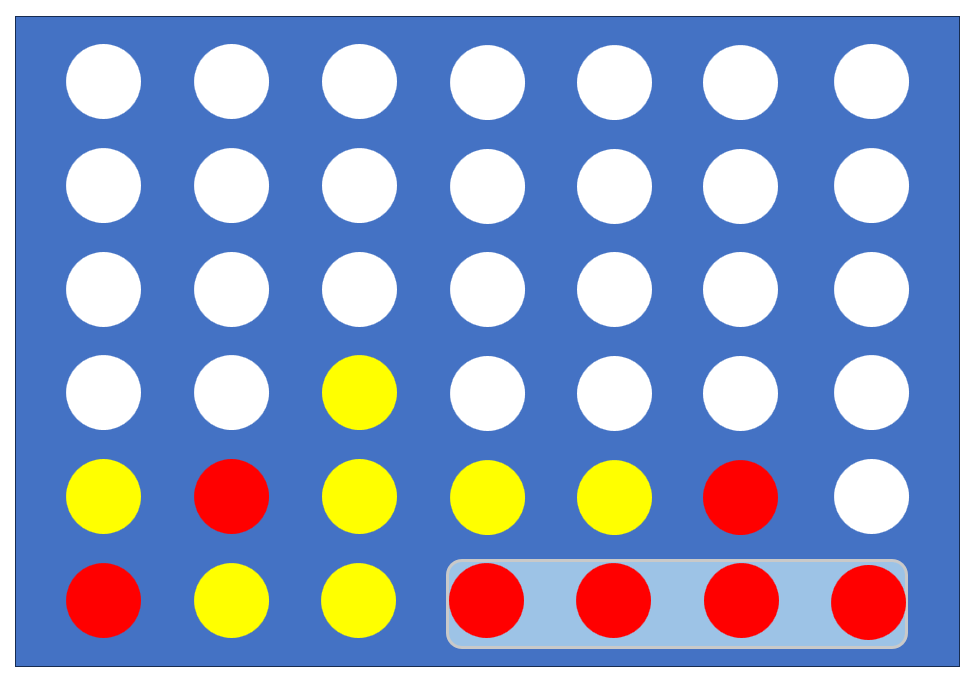
\includegraphics[width=0.8\linewidth]{images/Waagrecht}
	\caption[Vier rote Steine in Reihe waagrecht]{Vier rote Steine waagrecht im Raster}
	\label{fig:waagrecht}
\end{figure}
\begin{figure}[H]
	\centering
	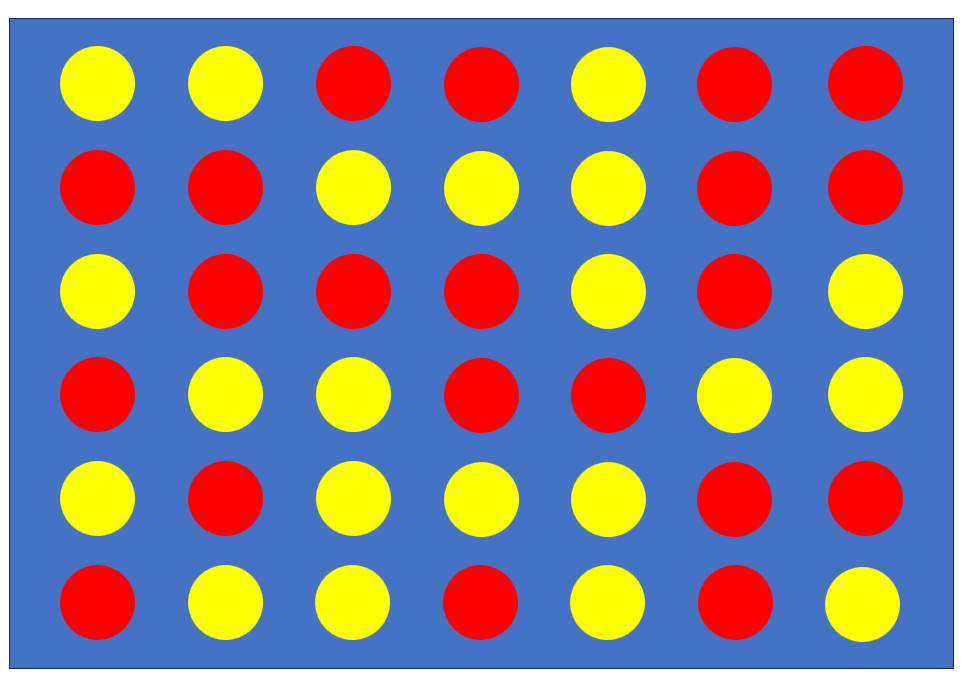
\includegraphics[width=0.8\linewidth]{images/Unentschieden}
	\caption[Unentschieden]{Unentschieden - es kam keine vierer Reihe zustande}
	\label{fig:unentschiedent}
\end{figure}
\newpage
\section{Historischer Hintergrund}
%Das Spiel “Vier Gewinnt” wurde 1973 von Howard Wexler und Ned Strongin entwickelt. Die Erstveröffentlichung erfolgte 1974 durch die Firma Milton Bradley, die im deutschsprachigen Raum als MB Spiele bekannt ist.
%Die Entwicklung des Spiels erfolgte durch die Strongin und Wexler Corporation in den USA. Obwohl der Preis der Erstausgabe nicht überliefert ist, wurde das Spiel schnell zu einem beliebten Strategiespiel.\\
%Eine interessante Entwicklung erfolgte bereits vor der Entstehung des klassischen Vier Gewinnt: 1967 erschien in den USA eine dreidimensionale Variante namens “Score Four”. Diese wurde 1974 in Deutschland von Ravensburger unter dem Namen “Sogo” vertrieben und war in der DDR als “Raummühle” bekannt.\\
%Das klassische Vier Gewinnt etablierte sich rasch als beliebtes Familienspiel und wurde über die Jahre in verschiedenen Varianten neu aufgelegt. Die Einfachheit der Regeln bei gleichzeitiger strategischer Tiefe trug maßgeblich zum anhaltenden Erfolg des Spiels bei.\\
%https://www.gameorama.ch/de/museum/spielmuseum/timeline/gewinnt?

Vier Gewinnt wurde 1973 von Howard Wexler und Ned Strongin entwickelt. Noch im selben Jahr lizenzierten die beiden Erfinder das Spiel an die Firma Milton Bradley, im deutschsprachigen Raum besser bekannt als ,,MB Spiele''
\autocite{gameorama_4gewinnt}\autocite{wikipedia_vier_gewinnt}.
Im darauffolgenden Jahr 1974 wurde das Spiel Vier Gewinnt von Milton Bradley veröffentlicht und in den Handel gebraucht. Das Spiel entwickelte sich seitdem zu einem der bekanntesten und beliebtesten Strategiespiele \autocite{wikipedia_vier_gewinnt}. Tatsächlich entwickelt es sich sogar zu einem echten Klassiker. Das Spiel ist beliebt bei Jung und Alt, da es recht leicht zu erlernen ist. Vier Gewinnt fördert die Konzentration und das logische Denken \autocite{50plus_vier_gewinnt}.

Im Jahr 1967 erschien in den USA eine dreidimensionale Variante vom Spiel Vier Gewinnt, unter dem Namen ,,Score Four''. In Deutschland brauchte die Firma Ravensburger 1974 eine dreidimensionale Variante mit dem Namen ,,Sogo'' auf den Markt. (siehe Abbildung:\ref{fig:Sogo}) \
1988 wurde das Spiel von Victor Allis und James D. Allen nahezu gleichzeitig und unabhängig voneinander vollständig gelöst. Die Beiden haben mathematisch bewiesen, dass der erste Spieler bei fehlerfreiem Spiel immer gewinnen kann, wenn er den ersten Stein in der mittleren Spalte platziert.\autocite{wikipedia_vier_gewinnt}.

%autocite{abebooks_image}
\begin{figure}[H]
	\centering
	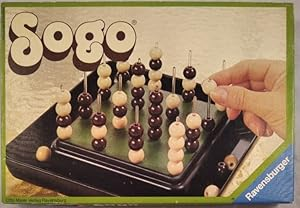
\includegraphics[width=0.8\linewidth]{images/Sogo}
	\caption[Sogo von Ravensburger \autocite{abebooks_image}]{dreidimensionale Variante ,,Sogo'' von Ravensburger}
	\label{fig:Sogo}
\end{figure}
\newpage
\section{Mathematische Eigenschaften des Spiels}
Das Spiel 4Gewinnt weist mehrere wichtige mathematische Eigenschaften auf, die für seine Analyse fundamental sind.\\
Hierbei liegt vorallem der Fokus auf Spielfeldgröße und Kombinatorik. Das klassische Spielfeld besteht aus 7 Spalten und 6 Reihen, was 42 mögliche Positionen ergibt. Diese Dimension wurde damals bewusst festgelegt, um ein ausgewogenes Verhältnis zwischen Komplexität und Spielbarkeit zu gewährleisten.\\

Die Gesamtzahl der theoretisch möglichen Spielzustände lässt sich wie folgt berechnen:
\begin{itemize}
	\item Jede Position kann drei Zustände annehmen: leer, Spieler 1, Spieler 2
	\item Dies ergibt theoretisch  mögliche Zustände\\
	
	Die tatsächliche Anzahl ist jedoch deutlich geringer, da:
	\item Spielsteine nur von unten nach oben gesetzt werden können
	\item Das Spiel endet, sobald vier Steine in einer Reihe liegen
	\item Nicht alle Kombinationen sind durch legale Spielzüge erreichbar
\end{itemize}

Komplexitätsgrad
•	Der durchschnittliche Verzweigungsfaktor (mögliche Züge pro Spielsituation) liegt bei etwa 4
•	Die maximale Spieltiefe beträgt 42 Züge
•	Die Spielbaumkomplexität ist deutlich geringer als bei Schach, aber höher als bei Tic-Tac-Toe
Symmetrieeigenschaften
Das Spielfeld weist eine vertikale Symmetrie auf, wodurch sich die Anzahl der zu analysierenden Positionen reduziert. Die mittlere Spalte nimmt dabei eine besondere strategische Position ein.
Diese mathematischen Eigenschaften bilden die Grundlage für die spieltheoretische Analyse und die Entwicklung von Lösungsstrategien.
\chapter{Spieltheoretische Grundlagen}

\section{Definition und Konzepte der Spieltheorie}
\section{Klassifikation von Spielen}
\section{Relevante spieltheoretische Konzepte für Vier Gewinn}
\chapter{Analyse von Vier Gewinnt aus spieltheoretischer Sicht}

%Die spieltheoretische Analyse von „Vier Gewinnt“ erfordert eine präzise und formale mathematische Darstellung des Spiels, um dessen strategische Struktur vollständig zu erfassen. Diese Darstellung ermöglicht es, die komplexen Entscheidungsprozesse der Spieler zu analysieren und optimale Strategien zu bestimmen. Im Wesentlichen gibt es zwei zentrale Darstellungsformen, die für die Analyse verwendet werden. Diese Darstellungsformen werden aufgezeigt und bewertet.
%

Die spieltheoretische Analyse des Spiels Vier Gewinnt erfordert eine systematische Untersuchung verschiedener strategischer Komponenten und mathematischer Aspekte. Im Folgenden Kapitel ,,Analyse von Vier Gewinnt aus spieltheoretischer Sicht'' werden die wesentlichen Elemente dieser Analyse detailliert dargestellt.
\section{Darstellung des Spiels in Normalform}
%
%Die Extensivform stellt das Spiel als Spielbaum dar und wird durch den Tupel  beschrieben T= (N,K,P,U,h,p), wobei:
%\begin{itemize}
%	\item N die Menge der Spieler (Spieler 1 und 2)
%	\item K die Menge aller Knoten (Spielpositionen)
%	\item P die Menge der Spielerpositionen
%	\item U die Menge der Endknoten
%	\item h die Auszahlungsfunktion
%	\item p die Vorgängerfunktion ist
%\end{itemize}
%Für Vier Gewinnt ist die Extensivform besonders geeignet, da sie die sequentielle Struktur des Spiels abbildet, die perfekte Information widerspiegelt und eine intuitive Analyse von Zugfolgen ermöglicht.

%*******Noch Ändern************************************************************************************
Die Normalform-Darstellung wird das Spiel als Zwei-Personen-Nullsummenspiel charakterisiert, bei dem der Gewinn eines Spielers den Verlusten des anderen bedeutet. 


Die Payoff-Matrix muss dabei die verschiedenen Spielsituationen und deren Ausgänge abbilden, wobei jeder Spieler in seiner Zugfolge bis zu sieben verschiedene Strategien pro Zug zur Verfügung hat

 \section{Darstellung des Spiels in Extensivform}
%Die Normalform hingegen repräsentiert das Spiel als Matrix G=(N,S,u) , mit:
%\begin{itemize}
%	\item N als Menge der Spieler
%	\item S als Menge der Strategieprofile
%	\item u als Auszahlungsfunktion
%\end{itemize}
%
%Die mathematische Beschreibung des Spielbaums erfolgt durch:
%T = (V,E,v_0) 
%wobei:
%\begin{itemize}
%	\item V die Menge aller Knoten
%	\item E die Menge der Kanten (mögliche Züge)
%	\item v_0 der Wurzelknoten (Ausgangsposition) ist
%\end{itemize}
%
%Die Darstellung in Normalform ist aufgrund der hohen Anzahl möglicher Strategien sehr umfangreich und für praktische Analysen weniger geeignet. Die Größe der Normalform-Matrix wächst exponentiell mit der Spieltiefe.

%*******Noch Ändern************************************************************************************
Der Spielbaum in der Extensivform zeigt die sequentielle Struktur des Spiels. Jeder Knoten repräsentiert eine Spielsituation, von der aus verschiedene Zugmöglichkeiten ausgehen. Die Teilspielanalyse ermöglicht es, einzelne Spielsituationen isoliert zu betrachten und optimale Strategien zu entwickeln5
. Bei perfektem Spiel beider Spieler ergeben sich dabei klare Strukturen, die durch den Zermelo'schen Bestimmtheitssatz beschrieben werden können

\section{Strategien und Gleichgewichte}
%*******Noch Ändern************************************************************************************
Die Analyse der Strategien zeigt, dass es im Vier Gewinnt dominante Strategien gibt. Nach dem Zermelo'schen Bestimmtheitssatz lässt sich das Spiel in eine von drei Kategorien einordnen, wobei sich herausgestellt hat, dass der erste Spieler eine dominante Strategie besitzt5
. Die Nash-Gleichgewichte manifestieren sich in den optimalen Zugfolgen, wobei die Kontrolle der zentralen Spalten eine entscheidende Rolle spielt2
.

\section{Komplexität des Spielbaums}
Die Komplexität des Spielbaums ist beträchtlich. Der Verzweigungsfaktor wird durch die sieben möglichen Züge pro Spielsituation bestimmt, wobei sich die Komplexität mit jeder Erhöhung der Baumtiefe multipliziert2
. Die computationellen Herausforderungen ergeben sich aus der Notwendigkeit, große Mengen von Spielzuständen zu analysieren und zu bewerten. Dabei müssen bestimmte Verhaltensregeln der Spieler berücksichtigt werden, wie etwa das sofortige Nutzen von Gewinnmöglichkeiten und das Verhindern gegnerischer Gewinnzüge2
. Die Analyse zeigt, dass trotz der scheinbaren Einfachheit der Spielregeln eine erhebliche mathematische Komplexität vorliegt. Die praktische Implementierung optimaler Strategien erfordert daher sowohl theoretisches Verständnis als auch effiziente Algorithmen zur Bewältigung des großen Zustandsraums. Besonders die Kontrolle strategisch wichtiger Positionen und die Fähigkeit, mehrere Züge vorauszudenken, sind entscheidend für den Spielerfolg2
.
	
\chapter{Lösungsansätze für Vier Gewinnt}
\chapter{Anwendung der Spieltheorie auf Vier Gewinnt}
\label{cha:Anwendung der Spieltheorie auf Vier Gewinnt}
In diesem Kapitel werden die spieltheoretischen Aspekte von 4Gewinnt, einschließlich der Analyse von Spielsituationen, der Berechnung von Gewinnwahrscheinlichkeiten und der Entwicklung von Spielstrategien untersucht.


\section{Analyse von Spielsituationen}
\label{sec:Analyse von Spielsituationen}
Für das Verständnis der Spieldynamik und die Entwicklung effektiver Strategien, ist die Analyse der Spielsituation entscheidend.
Vier Gewinnt, ist ein zwei Personen Spiel mit vollständiger Information. Das bedeutet, alle Spieler zu jeder Zeit den gesamten Zustand des Spiels kennen \autocite{ruile2009viergewinnt}.

Der Bestimmungssatz von Ernst Zermelo besagt, dass sich jedes kombinatorische Spiel in eine der folgenden Kategorien einordnen lässt.
\begin{enumerate}
	\item  Der beginnende Spieler hat eine dominante Strategie. Wenn das Spiel optimal, ohne Fehler verläuft, gewinnt er die Partie.
	\item Der nachziehende Spieler 2 hat eine dominante Strategie. Wenn das Spiel optimal verläuft, gewinnt dieser.
	\item Keiner der beiden Parteien hat eine dominante Strategie. Wenn beide Spieler optimal spielen, endet das Spiel ohne einen Sieger. Sobald ein Spieler einen Fehler macht, gewinnt der andere Spieler das Spiel \autocite{mueller_2011}.
\end{enumerate}
\\

Aus der Analyse geht hervor, dass bestimmte Situationen von besonderer Bedeutung für einen Sieg sind.
Das bilden einer horizontalen Viererreihe sind schwer zu erreichen. Umso wichtige ist es einen Sieg die Spalten 1-5 zu kontrollieren. 


\section{Berechnung von Gewinnwahrscheinlichkeiten}
Aufgrund der Komplexität des Spiels stellt die Berechnung der Gewinnwahrscheinlichkeit in Anwendung eine Herausforderung dar. Das Spielraster besteht aus sieben Spalten und sechs Zeilen, dadurch entsteht eine enorm große Anzahl an möglichen Zuständen. Was die Wahrscheinlichkeitsberechnung für den Gewinn des Spiels so komplex macht.
Moderne Ansätze zur Berechnung der Gewinnwahrscheinlichkeit greifen auf KI-Technik zurück. Die exakte Berechnung für alle möglichen Spielsituationen bleibt aufgrund der Komplexität von Vier Gewinnt eine Herausforderung \autocite{ruile2009viergewinnt}.
\section{Entwicklung von Spielstrategien}
	
Um eine gute Strategie für 4Gewinnt mit dem Alpha-Beta-Algorithmus zu entwickeln und später zu programmieren, müssen mehrere Schritte beachtet werden. Hier wird der Ansatz des gesamten Prozess kurz erläutert, von der Spielrepräsentation über die Bewertung von Stellungen bis hin zur Integration des Alpha-Beta-Algorithmus.

\subsection*{1. Spielfeld als Datenstruktur}
Zunächst muss das Spielfeld von 4Gewinnt in einer Form dargestellt werden, die von einem Algorithmus verarbeitet werden kann.
Hierzu kann ein 2D-Array (6 Zeilen × 7 Spalten) verwendet werden, das den Zustand des Spielfeldes beschreibt. Für jede Situation kann eine andere Zahl verwendet werden:
\begin{itemize}
	\item 0: Leeres Feld
	\item 1: Spielstein von Spieler 1
	\item -1: Spielstein von Spieler 2
\end{itemize}

Das Spielfeld kann nun als Array folgendermaßen dargestellt werden:

\[
\text{Spielfeld} =
\begin{pmatrix}
	0 & 0 & 0 & 0 & 0 & 0 & 0 \\
	0 & 0 & 0 & 0 & 0 & 0 & 0 \\
	0 & 0 & 0 & 0 & 0 & 0 & 0 \\
	0 & 0 & 0 & 0 & 0 & 0 & 0 \\
	0 & 0 & 0 & 0 & 0 & 0 & 0 \\
	0 & 0 & 0 & 0 & 0 & 0 & 0 \\
\end{pmatrix}
\]

\subsection*{2. Berechnung als Zugmöglichkeiten }
Da Spielsteine nur in den unteren freien Reihen platziert werden können, muss eine Funktion implementiert werden, die gültige Züge berechnet:

\begin{lstlisting}[language=Python, caption=Funktion zur Berechnung gültiger Züge]
	def gueltige_zuege(board):
	return [spalte for spalte in range(7) if brett[0][spalte] == 0]
\end{lstlisting}

\section*{3. Bewertung der Spielstellung}

Eine Bewertungsfunktion ist entscheidend für die Strategie. Sie schätzt den Wert einer Stellung ein und liefert eine Zahl:

\begin{itemize}
	\item \textbf{Gewinn für Spieler:} Sehr hoher Wert, z. B. \( +1000 \).
	\item \textbf{Verlust für Gegner:} Sehr niedriger Wert, z. B. \( -1000 \).
	\item \textbf{Potenzielle Verbindungen:} Punkte für 2er- und 3er-Reihen, die noch zu einem Sieg führen können.
	\item \textbf{Blockieren von Gegnerzügen:} Zusätzliche Punkte für Züge, die den Gegner daran hindern, 4 in eine Reihe zu bilden.
\end{itemize}

\section*{4. Alpha-Beta-Algorithmus implementieren}
	Der Alpha-Beta-Algorithmus wird verwendet, um den besten Zug zu berechnen, indem der Suchbaum effizient durchsucht wird. 
    Es geht darum, den besten Zug auszuwählen, basierend auf einer bestimmten Spielsituation und der Tiefe. Der Alpha-Beta-Algorithmus durchsucht den Entscheidungsbaum bis z.B. zur Tiefe 4 und nutzt alpha und beta, um unnötige Pfade auszulassen. maximizingPlayer=True gibt an, ob der Spieler seinen Vorteil maximiert.
\begin{lstlisting}[language=Python, caption=Alpha-Beta Algorithmus - Überblick]
	# Alpha-Beta Algorithmus in Aktion
	bester_Zug = alpha_beta(board, Tiefe=4, alpha=-float('inf'), beta=float('inf'), maximizingPlayer=True)
	print(f"Bester Zug: Spalte {bester_Zug}")
\end{lstlisting}

\section*{5. Entscheidung für den besten Zug}

Im fünften Schritt geht es darum, den optimalen Zug für den aktuellen Spieler zu finden. Dazu werden alle möglichen Züge angeschaut und mithilfe dem Alpha-Beta-Algorithmus bewertet. Der Zug, der am besten abschneidet – je nachdem, ob der Spieler versucht, seinen Punktestand zu maximieren oder zu minimieren – wird dann ausgewählt. Dieser Schritt ist entscheidend für die Entscheidungsfindung und markiert das Ende der Analyse des Spielbaums.

\begin{lstlisting}[language=Python, caption=Entscheidung für den besten Zug - Überblick]
# Grober Aufbau der Funktion zur Zugentscheidung
def bester_zug(board, tiefe, spieler):
bester_wert = float('-inf') if spieler == 1 else float('inf')
beste_spalte = None

for spalte in gueltige_zuege(board):
zug_wert = alpha_beta(anwenden_zug(brett, spalte, spieler), tiefe - 1, -float('inf'), float('inf'), False)
if (spieler == 1 und zug_wert > bester_wert) or (spieler == -1 und zug_wert < bester_wert):
bester_wert = zug_wert
beste_spalte = spalte

return beste_spalte
\end{lstlisting}
\begin{itemize}

	\item Die Funktion \texttt{bester\_zug} ist darauf ausgelegt, den besten Zug für einen Spieler zu bestimmen. 
	\item \texttt{gueltige\_zuege(board)} gibt alle gültigen Spalten zurück, in die ein Stein gesetzt werden kann. 
	\item \texttt{anwenden\_zug(board, spalte, spieler)} simuliert das Setzen eines Steins in eine bestimmte Spalte. 
	\item Der \emph{alpha-beta}-Algorithmus wird auf das simulierte Spielfeld angewendet, um die Bewertung des Zugs zu berechnen. 
	\item Der Spieler wählt den Zug mit der höchsten Bewertung (für Maximierer) oder der niedrigsten Bewertung (für Minimierer).
\end{itemize}

\section*{5. Endzustände erkennen}

Für die Auswertung der Endzustände wird eine Funktion benötigt, um festzustellen, ob das Spiel vorbei ist. Es können zwei Endzustände eintreffen:
\begin{itemize}
	\item Einer der Spieler hat 4 Steine in einer Reihe.
	\item Das Spielfeld ist voll.
\end{itemize}

Die Funktion Endzustand\_erreicht überprüft, ob ein Endzustand in einem Spiel erreicht wurde, indem sie zwei Bedingungen prüft: ob ein Spieler gewonnen hat (über die Funktion Spieler\_gewinnt) oder ob das Spielfeld voll ist (über die Funktion Board\_voll). 

\begin{lstlisting}[language=Python, caption=Erkennung des Endzustands]
def Endzustand_erreicht(board):
return Spieler_gewinnt(board) or Board_voll(board[0][spalte] != 0 for spalte in range(7))
\end{lstlisting}

\section*{7. Spielstrategie optimieren}

Nach dem Programmieren der Spielstrategien steht die Optimierung im Vordergrund. Um die Effizienz zu steigern, sollten Suchtiefe und Zeitlimit angepasst werden.

Die \textbf{Suchtiefe} kann je nach \textbf{Rechenleistung} variiert werden, um ein gutes Gleichgewicht zwischen der Tiefe des Spielbaums und der benötigten Rechenzeit zu finden. Da der Algorithmus auf einem LEGO Spike Roboter läuft, ist die Rechenzeit begrenzt. Daher ist es sinnvoll, eine Tiefensuche zu implementieren, die es ermöglicht, innerhalb eines festgelegten Zeitlimits die bestmögliche Tiefe zu erreichen. 








\chapter{Systementwurf}

Es soll eine detaillierte und funktionsfähige Vorrichtung entworfen werden, die in der Lage ist, Spielsteine präzise und zuverlässig in die vorgesehenen Spalten des Spielständers einzuführen. Dazu muss der Mechanismus so gestaltet sein, dass er unterschiedliche Positionen des Spielständers ansteuern und die Spielsteine mit der nötigen Genauigkeit platzieren kann. Nach dem Einwurf des Spielsteins muss die Vorrichtung den Spielständer wieder für den nächsten Zug freigeben, was eine genaue Steuerung und Rückkehr in die Ausgangsposition erfordert. Die mechanische Konstruktion muss robust und wiederholgenau arbeiten, um einen flüssigen und störungsfreien Spielablauf zu gewährleisten.


\section{Komponenten}
Zur Verwendung stehen folgende Sensorik und Aktorik zur Verfügung:


\begin{itemize}
	\item \textbf{großer LEGO® Technic Hub:}
	Der Hub ist das Steuerungselement des Spike Prime Systems. Er umfasst sechs Ein-/Ausgänge, welche den Anschluss von Peripheriegeräten, wie Sensorik und Aktorik, ermöglicht. Mit einem Micro-USB-Anschluss und Bluetooth wird die Kommunikation mit kompatiblen Endgeräten hergestellt. Der Hub besitzt ein integriertes MicroPython-Betriebssystem mit einem 100-MHz-Prozessor. 
	Weitere Ausstattungen sind:
	Individuell anpassbaren Lichtmatrix (5x5)
	Aufzeigen von wichtigen Informationen und Statusmeldungen
	Tasten
	Ermöglichen eine einfache Navigation und Steuerung durch Menüs 
	Lautsprecher
	6-achsigen Kreiselsensor
	
	\begin{figure}[H]
		\centering
		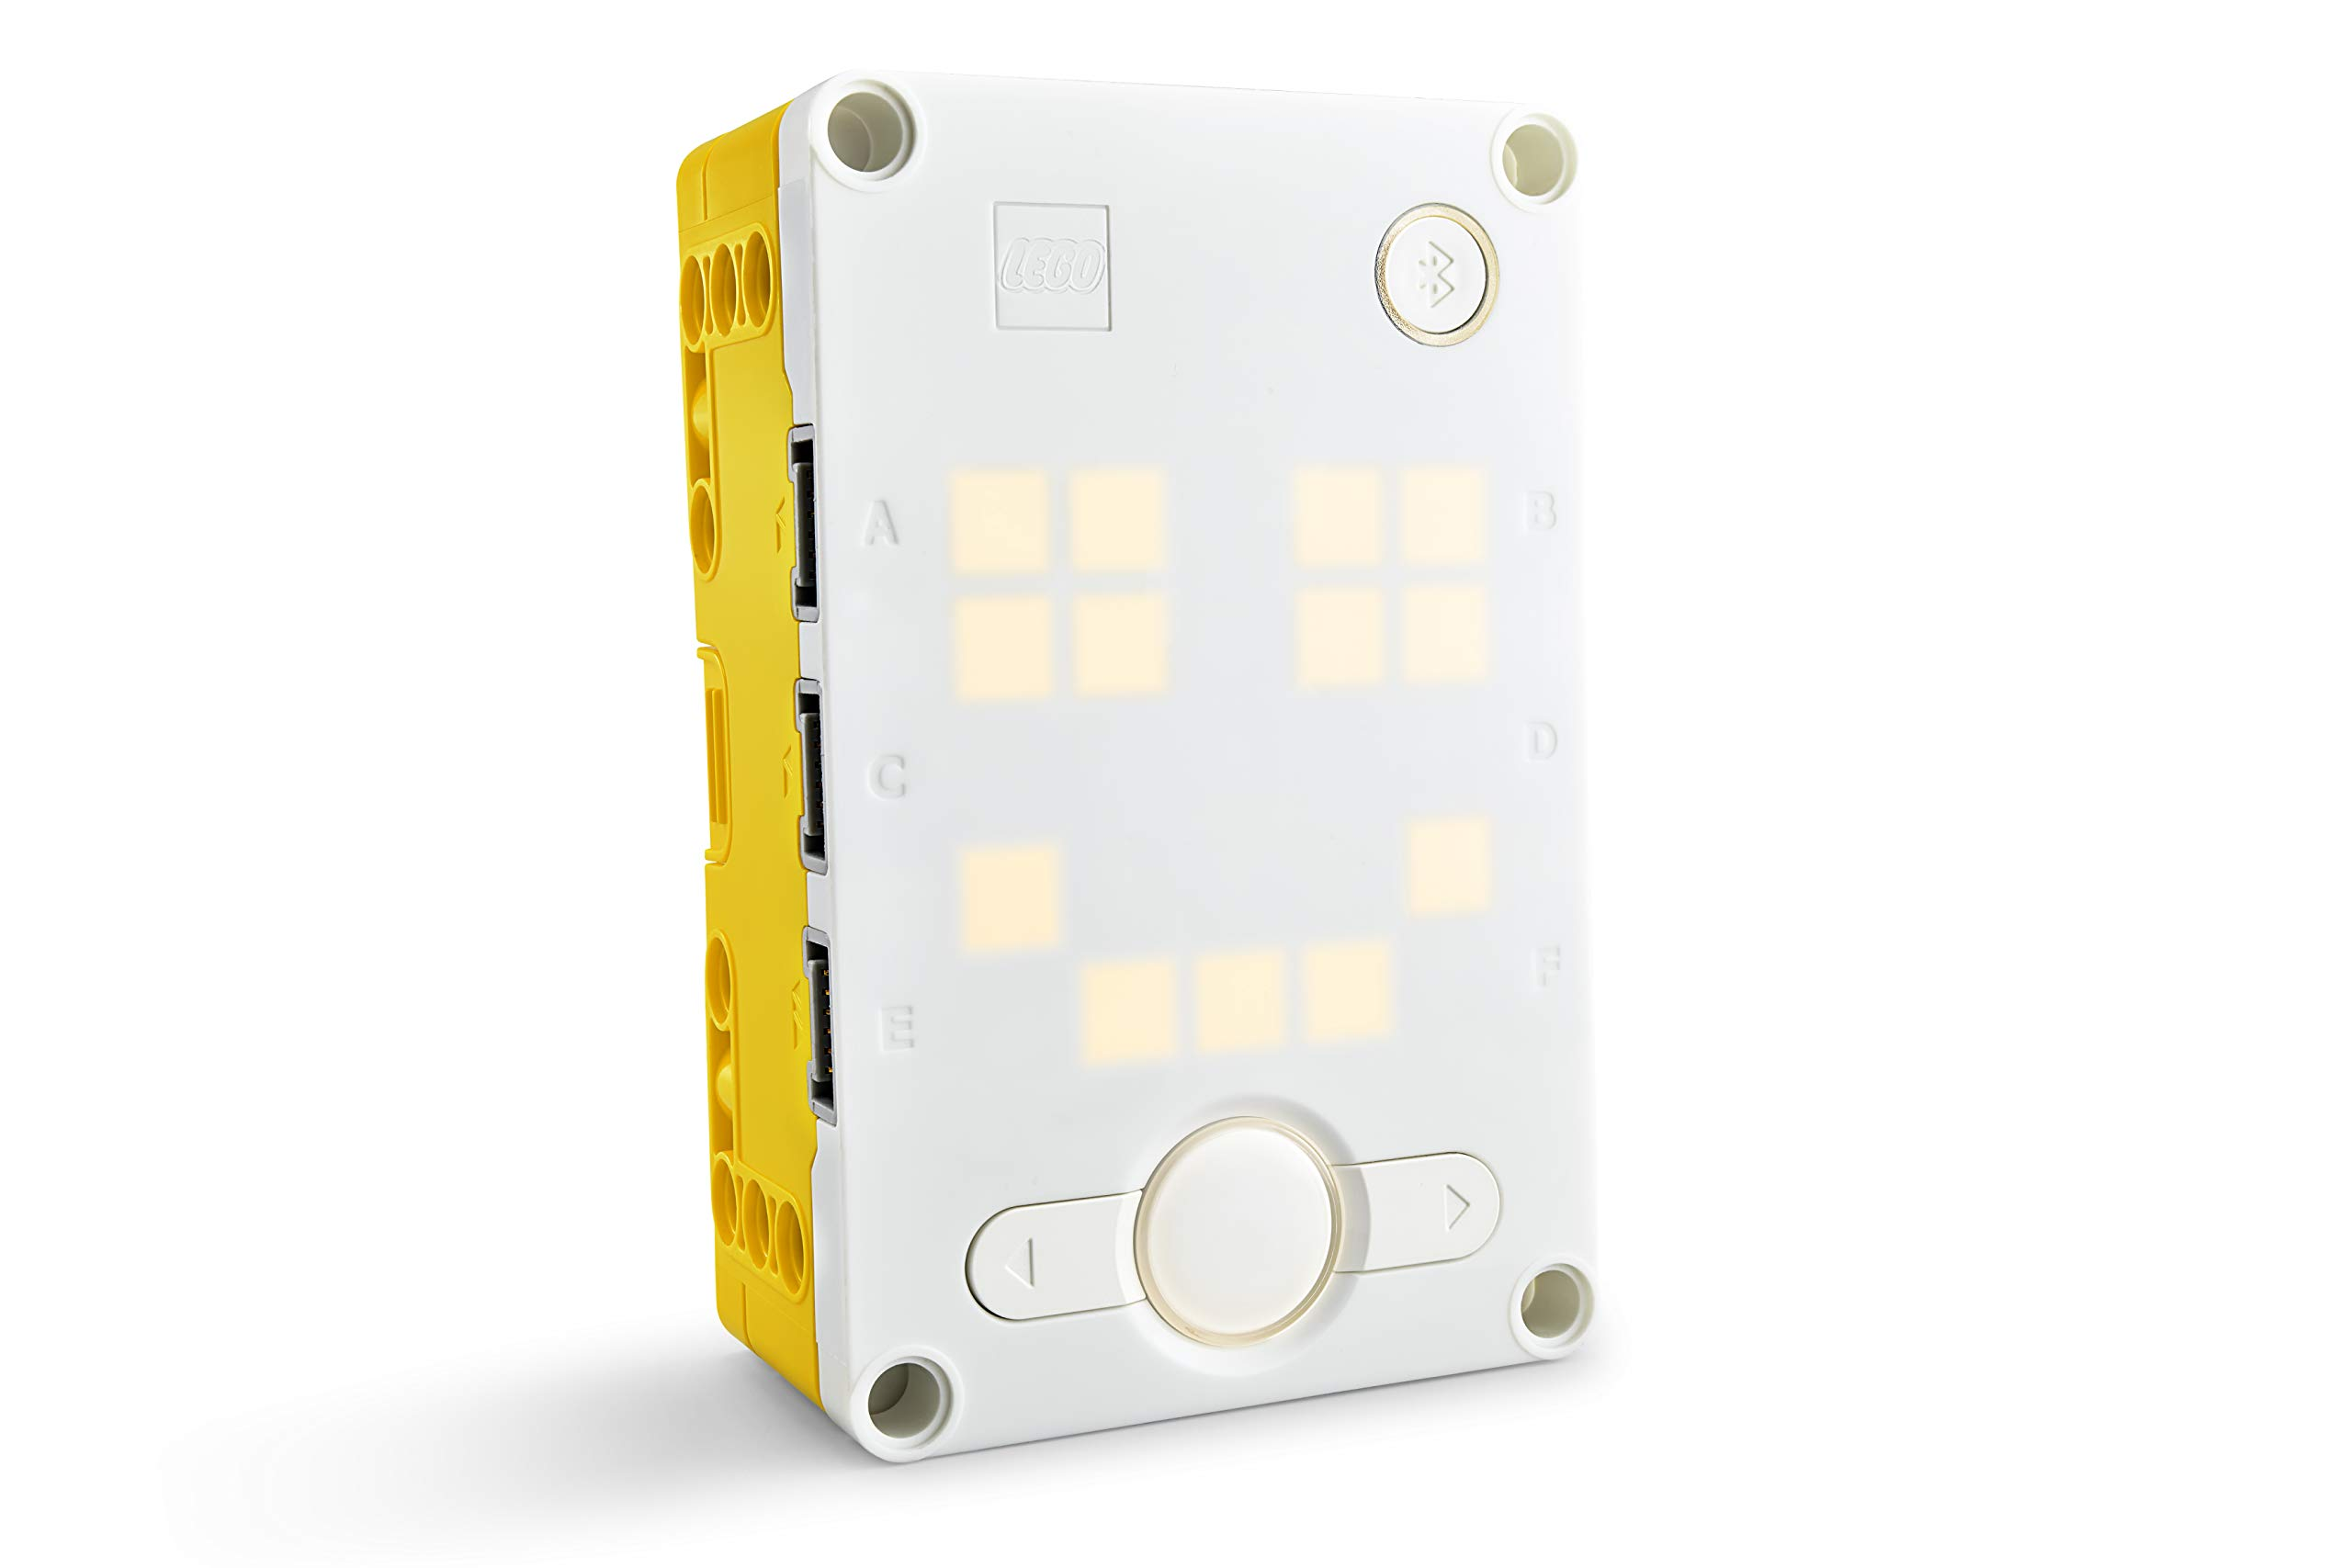
\includegraphics[width=0.5\linewidth]{images/Hub}
		\caption{Lego Technic Hub}
		\label{fig:hub}
	\end{figure}
	
	
	\item \textbf{LEGO® Technic Farbsensor:}
	Dieser Sensor kann durch die Intensität des reflektierten Lichts, welche er durch den eingebauten Lichtring erzeugt, bis zu acht Farben erkennen und unterscheiden (erkennbare Farben: schwarz, blau, rot, weiß, braun, gelb, pink und grün).  Er wird vor allem bei Anwendungen, wie Sortieren nach Farben, Linienverfolgung von farbigen Streifen und zum Ausführen von farbcodierten Befehlen eingesetzt. Um die Farberkennung optimal auf die entsprechende Umgebung anzupassen, wird das Umgebungslicht zuvor ausgewertet.
	
	\begin{figure}[H]
		\centering
		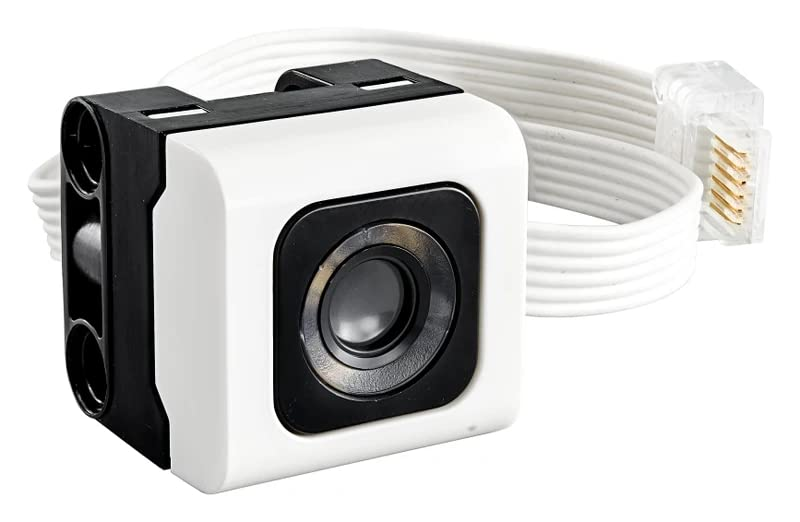
\includegraphics[width=0.5\linewidth]{images/Farbsensor}
		\caption{Lego Technic Farbsensor}
		\label{fig:farbsensor}
	\end{figure}
	
	
	\item \textbf{LEGO® Technic Großer Winkelmotor}
	Für die Bewegungssteuerung wird dieser Winkelmotor mit hoher Drehkraft und präziser Steuerung verwendet. Dieser Motor ist dafür ausgelegt, um schwere und komplexe Konstruktionen exakt in Geschwindigkeit und Position verfahren zu können. Dies wird durch den internen Winkel- und Rotationssensor ermöglicht. Der Anwendungsbereich ist vielseitig, unter anderem wird dies als Antrieb von Rädern, Gelenke, Greifarme, Hebevorrichtungen und Drehscheibe angewandt. Vor allem für Aufgaben, welche eine genau und wiederholbare Aktion ausüben müssen.
	
	\begin{figure}[H]
		\centering
		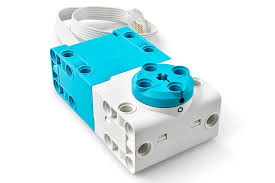
\includegraphics[width=0.5\linewidth]{images/Motor}
		\caption{Lego Technic Winkelmotor}
		\label{fig:motor}
	\end{figure}
	
\end{itemize}

\section{Zusammenspiel von Soft- und Hardware}

Der LEGO SPIKE Farbsensor eignet sich hervorragend zur Erkennung der Spielsteine in einem Vier-Gewinnt-Spiel. 

\subsection{Mechanische Konstruktion des Farbsensor-Systems}

Das Farbsensor-System basiert auf einem zweiachsigen Antriebssystem, das eine präzise Bewegung sowohl in vertikaler als auch in horizontaler Richtung ermöglicht. 

Die \textbf{vertikale Bewegung} wird durch eine Kettenkonstruktion realisiert, an der der Farbsensor befestigt ist. Ein LEGO SPIKE Motor treibt die Kette präzise an und sorgt dafür, dass der Sensor alle sechs Reihen des Spielfeldes abtasten kann. 

Die \textbf{horizontale Bewegung} erfolgt über einen Wagen mit vier Rädern. Dieser Wagen wird durch einen zweiten Motor angetrieben, der mit Encoderwerten für eine präzise Positionierung gesteuert wird. Durch die horizontale Bewegung können alle sieben Spalten des Spielfeldes abgedeckt werden.

Die \textbf{Steuerung der Bewegungen} erfolgt durch eine koordinierte Ansteuerung beider Achsen, wodurch der Farbsensor schrittweise von Position zu Position bewegt wird. Optimierte Verfahrwege minimieren die Scanzeit, und eine Kalibrierung der Positionen gewährleistet eine genaue Ausrichtung des Sensors.

Diese mechanische Konstruktion ermöglicht eine zuverlässige und präzise Abtastung aller 42 Spielfeldpositionen des Vier-Gewinnt-Spiels und stellt somit eine optimale Grundlage für die Umsetzung  dar.

\chapter{Zusammenfassung}


Die spieltheoretische Analyse von 4Gewinnt hat gezeigt, dass das Spiel trotz seiner scheinbaren Einfachheit eine hohe strategische Tiefe besitzt. Durch die Anwendung von Algorithmen wie Minimax und dessen Optimierung durch den Alpha-Beta-Algorithmus können optimale Entscheidungen getroffen werden, um entweder zu gewinnen oder ein Unentschieden zu erzwingen. Aber auch verschiedene Strategien haben einen Einfluss auf den Spielverlauf.

Der Alpha-Beta-Algorithmus ist hierbei besonders hervorzuheben, da er durch die effiziente Kürzung des Suchbaums eine präzise Analyse in kürzerer Zeit ermöglicht. Diese Eigenschaft ist für die praktische Umsetzung auf ressourcenbeschränkten Systemen wie dem LEGO SPIKE Roboter entscheidend. Der Algorithmus gewährleistet, dass der Roboter in der Lage ist, komplexe Spielsituationen in Echtzeit zu bewerten und optimale Züge zu berechnen.

Mit den gewonnenen Erkenntnissen aus der Spieltheorie und ist nun der Grundstein für den zweiten Teil dieser Studienarbeit gelegt. In diesem Teil wird ein Programm entwickelt, das den Alpha-Beta-Algorithmus implementiert und mit der Hardware des LEGO SPIKE Roboters zusammenarbeitet. 




% ---- Literaturverzeichnis ----------
\interlinepenalty 10000					% Verhindert einen Umbruch mitten in Literatureinträgen
\printbibliography						% Erstellen des Literaturverzeichnisses
\clearpage

% -----Ausgabe aller Verzeichnisse ---
\setlength{\parskip}{0.5\baselineskip}

% Alle Abkürzungen, die in der Arbeit verwendet werden. Die Alphabetische Sortierung übernimmt Latex. Nachfolgend sind Beispiele genannt, welche nach Bedarf angepasst, gelöscht oder ergänzt werden können.
% Die Angaben in der eckigen Klammer werden zur Sortierung der Einträge verwendet. Vor allem bei Formelzeichen hat man sonst das Problem, dass diese möglicherweise nicht wie gewünscht sortiert werden.

% Bei den unten stehenden Formelzeichen ist erläutert, wie explizite Sortierschlüssel über den Inhalt der eckigen Klammer angegeben werden.

% Zum Aktualisieren des Abkürzungsverzeichnisses (Nomenklatur) bitte auf der Kommandozeile folgenden Befehl aufrufen :
% makeindex <Dateiname>.nlo -s nomencl.ist -o <Dateiname>.nls
% Oder besser: Kann in TexStudio unter Tools-Benutzer als Shortlink angelegt werden
% Konfiguration unter: Optionen-Erzeugen-Benutzerbefehle: makeindex -s nomencl.ist -t %.nlg -o %.nls %.nlo

% Allgemeine Abkürzungen %%%%%%%%%%%%%%%%%%%%%%%%%%%%
%\nomenclature[Abb]{Abb.}{Abbildung}
%\nomenclature[bzw]{bzw.}{beziehungsweise}
%\nomenclature[DHBW]{DHBW}{Duale Hochschule Baden-Württemberg}
%\nomenclature[ebd]{ebd.}{ebenda}
%\nomenclaturev[etal]{et al.}{at alii}
\nomenclature[etc]{etc.}{et cetera}
%\nomenclature[evtl]{evtl.}{eventuell}
\nomenclature[f]{f.}{folgende Seite}
\nomenclature[ff]{ff.}{fortfolgende Seiten}
%\nomenclature[ggf]{ggf.}{gegebenenfalls}
%\nomenclature[Hrsg]{Hrsg.}{Herausgeber}
%\nomenclature[Tab]{Tab.}{Tabelle}
%\nomenclature[ua]{u. a.}{unter anderem}
%\nomenclature[usw]{usw.}{und so weiter}
\nomenclature[vgl]{vgl.}{vergleiche}
\nomenclature[zB]{z. B.}{zum Beispiel}
%\nomenclaturev[zT]{z. T.}{zum Teil}

% Dateiendungen %%%%%%%%%%%%%%%%%%%%%%%%%%%%%%%%%%%%
\nomenclature[EMF]{EMF}{Enhanced Metafile}
\nomenclature[JPG]{JPG}{Joint Photographic Experts Group}
\nomenclature[KI]{KI}{Künstliche Intelligenz}
\nomenclature[PDF]{PDF}{Portable Document Format}
\nomenclature[PNG]{PNG}{Portable Network Graphics}
%\nomenclature[]{XML}{Extensible Markup Language}

% Abkürzungen von Fachbegriffen %%%%%%%%%%%%%%%%%%%%
\nomenclature[ABS]{ABS}{Antiblockiersystem}
\nomenclature[ESC]{ESC}{Electronic Stability Control, Fahrdynamikregelung}

% Formelzeichen %%%%%%%%%%%%%%%%%%%%%%%%%%%%%%%%%%%%
\nomenclature[a]{$a$}{Beschleunigung}
\nomenclature[F]{$F$}{Kraft}
\nomenclature[m]{$m$}{Masse}
\nomenclature[P]{$P$}{Leistung}
\nomenclature[U]{$U$}{Spannung}
\nomenclature[R]{$R$}{Widerstand}


				% Datei mit allgemeinen Abkürzungen laden
\renewcommand{\nomname}{Verzeichnis verwendeter Formelzeichen und Abkürzungen}
%\addcontentsline{toc}{chapter}{\nomname}
\setlength{\nomlabelwidth}{.20\hsize}
\renewcommand{\nomlabel}[1]{#1 \dotfill}
\setlength{\nomitemsep}{-\parsep}
\printnomenclature						% Erzeugen des Abkürzungsverzeichnises, siehe auch Inhalt der Datei pages/abkuerzungen.tex
\clearpage

\listoffigures 							% Erzeugen des Abbildungsverzeichnisses 
\clearpage

\listoftables 							% Erzeugen des Tabellenverzeichnisses
\clearpage

% -----Anhang ------------------------

\appendix
%\pagenumbering{Roman}					% große, römische Seitenzahlen für Anhang, falls gewünscht
%\addchap{A Nutzung von Künstliche Intelligenz basierten Werkzeugen}
\setcounter{chapter}{1}

Im Rahmen dieser Arbeit wurden Künstliche Intelligenz (KI)\index{Künstliche Intelligenz} basierte Werkzeuge benutzt. Tabelle~\ref{tab:anhang_uebersicht_KI_werkzeuge} gibt eine Übersicht über die verwendeten Werkzeuge und den jeweiligen Einsatzzweck.

\begin{table}[hbt]	
	\centering
	\renewcommand{\arraystretch}{1.5}	% Skaliert die Zeilenhöhe der Tabelle
	\captionabove[Liste der verwendeten Künstliche Intelligenz basierten Werkzeuge]{Liste der verwendeten KI basierten Werkzeuge}
	\label{tab:anhang_uebersicht_KI_werkzeuge}
	\begin{tabular}{>{\raggedright\arraybackslash}p{0.3\linewidth} >{\raggedright\arraybackslash}p{0.65\linewidth}}
		\textbf{Werkzeug} & \textbf{Beschreibung der Nutzung}\\
		\hline 
		\hline
		ChatGPT & 	\vspace{-\topsep}
		\begin{itemize}[noitemsep,topsep=0pt,partopsep=0pt,parsep=0pt] 
			\item Grundlagenrecherche zu Spieltheorie 
			
		\end{itemize} \\
		Perplexity &	\vspace{-\topsep}
		\begin{itemize}[noitemsep,topsep=0pt,partopsep=0pt,parsep=0pt] 
			\item Grundlagenrecherche zu Spieltheorie 
			\item Formulierungshilfe
		\end{itemize} \\ 
		DeepL	&	\vspace{-\topsep}
		\begin{itemize}[noitemsep,topsep=0pt,partopsep=0pt,parsep=0pt] 
			\item Unterstützung beim Übersetzung von Abstract
		\end{itemize} \\ 
		Languagetool &	\vspace{-\topsep}
		\begin{itemize}[noitemsep,topsep=0pt,partopsep=0pt,parsep=0pt] 
			\item Formulierungshilfe 
			\item Rechtschreibkorrektur 
		\end{itemize} \\ 
	
	
		\hline 
	\end{tabular} 
\end{table}
\clearpage

%\		% Zeile auskommentieren bei finalem Dokument!


%\renewcommand{\glossaryname}{Glossar}
%\printglossaries
%\addcontentsline{toc}{chapter}{\glossaryname}

%\renewcommand{\indexname}{Sachwortverzeichnis}
%\printindex								% Erzeugen des Sachwortverzeichnisses

%%---------Notizen---------------------------
%\chapter*{Besprechungsnotizen}

\section{9.Oktober.2024}

\begin{itemize}
	\item Spieletheorie erfassen
	\item Speicherplatz im uController wird begrenzt sein
	\item Spielalgorithmus (wann wird geschaut wo Steine liegen - immer das ganze Feld abcannen?)
	\item Zeitplan erstellen
	\item  https://education.lego.com/de-de/downloads/spike-app/software/
	\item 
\end{itemize}

%	\chapter*{Anforderungsliste}
	\begin{table}[hbt]
	\centering
	%\captionabove{Tabelle mit wenig Inhalt}
	\label{Anforderungsliste}
	\begin{tabular}{ccc}
		\textbf{Nr} & \textbf{Anforderung an das System} & \textbf{F/W} \\
		\textbf{} & \textbf{}& \textbf{}  \\
		\hline
		\hline
		\textbf{} & \textbf{Allgemein}& \textbf{}  \\
		\hline
		\hline
		- & Lage der Steine erkennen & F\\
		\hline
		- & Das Ende des Speils erkennen & F\\
		\hline
		- & Beweglich - Steine in jede Spalte	& F\\
		\hline
		- &Magazin für Steine  & F\\
		\hline
		- &  & F\\
		\hline
		- &  & F\\
		\hline
		
	\end{tabular}
\end{table}

\end{document}